% !TeX root = ../thuthesis-example.tex

\chapter{引言}


\section{研究背景}

互联网自诞生以来,随着数十年的发展,已经成为了最重要的信息化基础设施。如图~\ref{fig:网民规模和互联网普及率}所示,从我国互联网络发展状况的统计报告\cite{cac.gov}中可以看出:“截至2020 年12 月,我国的移动网民用户规模已经累计达到9.88 亿,互联网的网络普及率已经高达70.4\%”。
% 如图所示,我们从有关我国互联网络发展状况的统计报告\cite{cac.gov}中可以看出:“截至2020 年6 月, 我国的移动网民用户规模已经累计达到9.40 亿, 互联网的网络普及率已经高达67.0\%”。
互联网的主要应用领域已经包括即时移动通信、搜索结果引擎、网络即时新闻、线下线上教育、购物以及出行等各个方面,可以说如今互联网已经和每一个人的工作和日常生活息息相关。



\begin{figure}
    \centering
    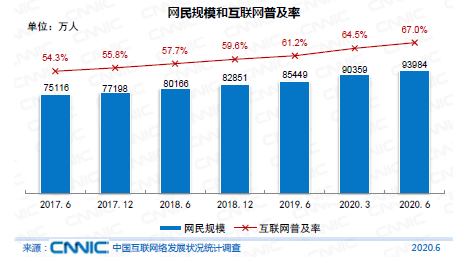
\includegraphics[width=0.6\linewidth]{网民规模.PNG}
    \caption{网民规模和互联网普及率}
    \label{fig:网民规模和互联网普及率}
  \end{figure}

随着网络重要性的提升、用户规模的膨胀,管理网络的难度也越来越大。网络系统繁琐而又复杂,它的设计、运营以及维护都必须依靠专业的网络运维技术人员。早期的网络运维管理工作绝大多数都是由运维工作人员手工操作来完成,此后人们逐渐发现一些重复性的工作可以用自动化脚本来实现,于是诞生了自动化运维。可以认为自动化的运维系统是一种建立在专家经验和人为制订规则之上的系统。但是随着互联网规模迅速增长,以及其服务种类和方式的日益多样化,人为设定基础运维规则的方法与技术渐渐难以应付大规模网络的运维需求。在此情况下,智能运维应运而生,与自动化运维仰仗专门人员的知识、人为制定规则不同,智能运维的着重点在于使用机器学习算法,先从庞大的运维管理数据中反复吸收经验进行学习,然后有条不紊的逐步提取规则。

% 随着网络重要性的提升、用户规模的膨胀,管理网络的难度也越来越大。网络是一个复杂的系统,它的部署、运行和维护都需要专业的运维人员。
% 早期的运维工作大部分是由运维人员手工完成,此后人们逐渐发现一些重复性的工作可以用自动化脚本来实现,于是诞生了自动化运维。自动化运维可以被认为是基于专家经验、人为制定规则的系统。
% 但是随着互联网规模急剧膨胀,以及服务类型的多样化,简单的、基于人为制定规则的方法并不能解决大规模运维的问题,因此产生了智能运维。与自动化运维依赖专家知识、人工生成规则不同,
% 智能运维强调使用机器学习算法从海量运维数据中不断学习、不断提炼规则。

异常检测是智能运维的关键环节,具有至关重要的意义。从网络故障管理的角度来说,做好异常检测可以提前预测故障的发生;从性能管理的角度来说,可以发现性能不佳的区域,避免因误配置、架构不合理导致性能下降;
从安全管理的角度来说,在网络攻击的前期阶段,及时发现并预警后续攻击,进而做出防御措施。因此,在复杂的网络环境中甄别出有效和异常流量尤为重要:在重大事故发生前,根据各项流量特征的变化,提前预测出即将发生的事故,提高应急响应速度,防患于未然。


本文以校园网为研究对象,进行网络流量异常检测算法和系统的研究。清华大学校园网是全球规模最大、架构最复杂、流量场景最多变的校园网之一,具有以下几个特点:
\begin{enumerate}
    \item 用户规模大,流量峰值高。清华大学校园网每天有10万台设备活跃在线,峰值时段同时在线设备约为7万台,流量约为30Gbps,图~\ref{fig:用户流量变化图}展示了一周内的用户流量变化情况。
    \item	用户应用类型多。如图~\ref{fig:用户应用类型图}所示,清华大学校园网中的用户应用类型远比一般的企业网复杂,在该网络环境中同时存在着几百种应用,这给数据分析带来了很多困难。
    \item	异常流量是常态。扫描流量、攻击流量占比多。
\end{enumerate}

\begin{figure}
  \centering
  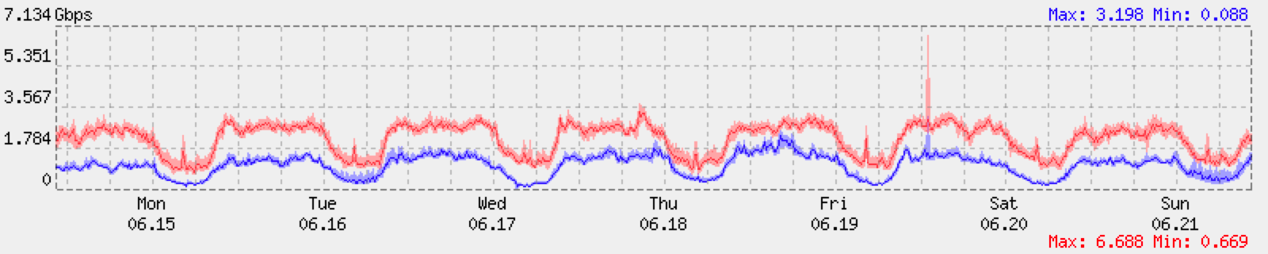
\includegraphics[width=0.6\linewidth]{用户流量变化图.png}
  \caption{用户流量变化图}
  \label{fig:用户流量变化图}
\end{figure}

\begin{figure}
  \centering
  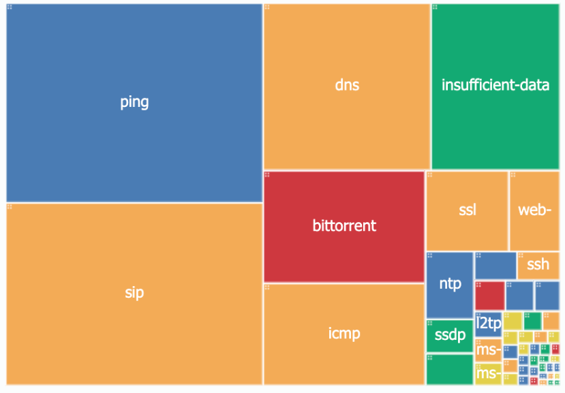
\includegraphics[width=0.6\linewidth]{用户应用类型图.png}
  \caption{用户应用类型图}
  \label{fig:用户应用类型图}
\end{figure}
% 接下来我们将以校园网为例,进行异常检测算法和系统的研究。清华大学校园网是全球规模最大,架构最复杂,流量场景最多变的校园网之一,具有以下几个特点:
% 1.	用户规模大,流量峰值高。每天有10万台设备活跃在线,同时在线设备最多为7万台,峰值流量约为30Gbps/s.
% 2.	用户应用类型多,远比一般的企业网复杂,在网络环境中几百种应用同时使用,这给数据分析带来了很多困难。
% 3.	异常流量是常态。扫描流量、攻击流量占比多。
% 这些特点给异常检测的研究和实现带来了诸多挑战。

% \section{研究内容}
% 围绕1.1节中提到的清华大学校园网流量异常检测的特点和挑战,本文分别展开了以下三方面研究:首先分析对比了开源数据集与


\section{论文的研究内容}
围绕1.1节中提到的清华大学校园网流量异常检测的特点和挑战,本文分别展开了以下几方面的研究:
\begin{enumerate}
  \item 本文分析对比了流量异常检测领域的两个经典开源数据集UNSW-NB15和CICIDS2017,引入了清华大学校园网的真实数据集,并且分别在这几个数据集上对现有的异常检测算法进行了实验对比。
  \item 在现有算法的基础上,本文将特征关系引入到神经网络的训练中,提出了一种基于特征关系图的循环神经网络算法(FG-RNN,Feature Graph-Recurrent Neural Network)。在复杂的网络流量环境下,流量特征种类繁多,且特征之间的相关性会随着流量变化而变化。原有的异常检测算法通常直接利用提取的特征进行训练,本文提出的FG-RNN算法有效利用了特征之间的相关性信息。
  \item 本文对基于特征关系图的循环神经网络算法进行了流式改造,使之能够满足实时异常检测的需求。为了应对海量的校园网流量数据和高速数据流,本文设计了一个基于Spark Streaming的实时异常检测系统。该系统分为输入模块、模型模块、检测模块三部分:输入模块负责将流量数据进行窗口划分、特征选择、特征抽取、合并计算;模型模块负责训练特征矩阵和关系矩阵,同时会周期性更新模型中的参数以避免模型效果衰减过快;检测模块负责对当前流量进行判别,并给出异常流量的类别。
  \item 本文对上述系统检测出的端口扫描进行了定量分析,发现其不仅是安全问题,同时会对无线网性能产生影响,严重时会造成100ms以上的时延增加。最后本文提出了两种优化策略,可以有效地缓解该问题。

\end{enumerate}

\section{论文内容和组织结构}
第1章为引言,主要介绍本文的研究背景以及研究内容。

第2章主要介绍网络流量异常检测的相关综述以及数据集分析对比。第2章首先对网络流量异常的定义和分类进行了介绍;接下来介绍了基于不同原理的常用异常检测算法;然后重点介绍了本文提出的算法所依赖的模型:循环神经网络模型;然后分析对比了开源数据集与校园网真实数据集,并且在多个数据集上对现有的算法进行了实验对比,指出了现有的异常检测算法在校园网流量环境下存在的主要问题。
% 最后,指出了现有的异常检测算法在当前大规模流量环境下存在的主要问题。

第3章至第5章是本文的主要研究内容。第3章首先对现有算法的不足进行了详细分析,然后提出了基于特征关系图的循环神经网络算法,并进行了算法性能评估。第4章设计并实现了一个基于Spark Streaming的流式处理系统,介绍了各个模块实现的架构和流程,对系统运行结果进行了分析。第5章研究了端口扫描问题对无线网性能的具体影响,并且提出了两种优化策略,均可有效地缓解端口扫描造成的性能问题。

最后,第6章对全文进行了总结,并且提出了未来展望。
